\documentclass[12pt,a4paper]{amsart}
\usepackage[utf8]{inputenc}
\usepackage[T1]{fontenc}
\usepackage{amsmath,amsfonts,amssymb}
\usepackage{tikz}
\usepackage{algorithm}
\usepackage{algorithmic}
\usepackage{listings}
\usepackage{xcolor}
\usepackage{geometry}
\usepackage{fancyhdr}
\usepackage{enumitem}
\usepackage{booktabs}
\usepackage{multirow}
\usepackage[hidelinks,bookmarksnumbered,bookmarksopen]{hyperref}
\usepackage{xeCJK}
\setCJKmainfont{LXGW WenKai}


% 页面设置
\geometry{left=2cm,right=2cm,top=2.5cm,bottom=2.5cm}
\pagestyle{fancy}
\fancyhf{}
\fancyhead[L]{图论复习总结}
\fancyhead[R]{\thepage}

% TikZ库
\usetikzlibrary{arrows,positioning,shapes,calc,trees,graphs}

% 代码高亮设置
\lstset{
    language=C++,
    basicstyle=\ttfamily\small,
    keywordstyle=\color{blue}\bfseries,
    commentstyle=\color{green!60!black},
    stringstyle=\color{red},
    numbers=left,
    numberstyle=\tiny\color{gray},
    stepnumber=1,
    numbersep=10pt,
    backgroundcolor=\color{gray!10},
    frame=single,
    tabsize=4,
    captionpos=b,
    breaklines=true,
    breakatwhitespace=false,
    showspaces=false,
    showstringspaces=false,
    showtabs=false
}

% 定理环境
\newtheorem{definition}{定义}[section]
\newtheorem{theorem}{定理}[section]
\newtheorem{algorithm_desc}{算法}[section]

\title{\textbf{数据结构第六章:图论复习总结}}
\author{期末考试复习资料}
\date{\today}

\begin{document}

% \maketitle

% % 目录设置
% \tableofcontents
% \newpage

\section{图的基本概念}

\subsection{图的定义}

\begin{definition}[图]
图是由顶点的有穷非空集合和顶点之间边的集合组成,通常表示为:
$$G = (V, E)$$
其中$G$表示一个图,$V$是顶点集合,$E$是边集合。
\end{definition}

\begin{center}
\begin{tikzpicture}[scale=1.2]
    % 无向图示例
    \node[circle,draw,minimum size=0.8cm] (v0) at (0,0) {$v_0$};
    \node[circle,draw,minimum size=0.8cm] (v1) at (2,1) {$v_1$};
    \node[circle,draw,minimum size=0.8cm] (v2) at (2,-1) {$v_2$};
    \node[circle,draw,minimum size=0.8cm] (v3) at (4,0) {$v_3$};
    
    \draw (v0) -- (v1);
    \draw (v0) -- (v2);
    \draw (v1) -- (v3);
    \draw (v2) -- (v3);
    \draw (v1) -- (v2);
    
    \node at (2,-2) {\textbf{无向图}};
    
    % 有向图示例
    \begin{scope}[xshift=6cm]
        \node[circle,draw,minimum size=0.8cm] (u0) at (0,0) {$u_0$};
        \node[circle,draw,minimum size=0.8cm] (u1) at (2,1) {$u_1$};
        \node[circle,draw,minimum size=0.8cm] (u2) at (2,-1) {$u_2$};
        \node[circle,draw,minimum size=0.8cm] (u3) at (4,0) {$u_3$};
        
        \draw[-latex] (u0) -- (u1);
        \draw[-latex] (u0) -- (u2);
        \draw[-latex] (u1) -- (u3);
        \draw[-latex] (u2) -- (u3);
        \draw[-latex,bend left] (u1) to (u2);
        
        \node at (2,-2) {\textbf{有向图}};
    \end{scope}
\end{tikzpicture}
\end{center}

\subsection{图的基本术语}

\begin{itemize}
    \item \textbf{邻接}:若存在边$(v_i, v_j)$,则称$v_i$和$v_j$互为邻接点
    \item \textbf{关联(依附)}:顶点$v$和边$e$相关联,称边$e$依附于顶点$v$
    \item \textbf{度}:
    \begin{itemize}
        \item 无向图:顶点$v$的度$TD(v)$是依附于该顶点的边数
        \item 有向图:入度$ID(v)$ + 出度$OD(v)$
        \item 悬挂顶点:度为1的顶点
        \item 孤立顶点:度为0的顶点
    \end{itemize}
    \item \textbf{路径与回路}:
    \begin{itemize}
        \item 路径:顶点序列$v_p = v_{i_0}v_{i_1}\cdots v_{i_m} = v_q$
        \item 路径长度:路径上边的数目
        \item 简单路径:顶点不重复的路径
        \item 回路(环):第一个和最后一个顶点相同的路径
        \item 简单回路:除第一个和最后一个顶点外,其余顶点不重复的回路
    \end{itemize}
    \item \textbf{连通性}:
    \begin{itemize}
        \item 连通:任意两顶点间都有路径的无向图
        \item 连通分量:无向图中的极大连通子图
        \item 强连通:任意两顶点间都有路径的有向图
        \item 强连通分量:有向图中的极大强连通子图
    \end{itemize}
    \item \textbf{特殊图类型}:
    \begin{itemize}
        \item 完全图:任意两个顶点之间都有边的简单图
        \item 无向完全图:$n$个顶点的完全图有$\frac{n(n-1)}{2}$条边
        \item 有向完全图:$n$个顶点的完全图有$n(n-1)$条弧
        \item 树:$n$个顶点$n-1$条边的连通无向图
        \item 森林:若干棵不相交树的集合
    \end{itemize}
\end{itemize}

\subsection{重要数学性质}

\begin{theorem}[握手定理]
在具有$n$个顶点$e$条边的无向图中:
$$\sum_{i=0}^{n-1} TD(v_i) = 2e$$
\end{theorem}

\begin{theorem}[有向图度数性质]
在具有$n$个顶点$e$条边的有向图中:
$$\sum_{i=0}^{n-1} ID(v_i) = \sum_{i=0}^{n-1} OD(v_i) = e$$
\end{theorem}

\section{图的存储结构}

\subsection{邻接矩阵}

\begin{definition}[邻接矩阵]
用$n \times n$的二维数组存储图,其中$A[i][j] = 1$表示存在边$(v_i, v_j)$。
\end{definition}

\begin{center}
\begin{tikzpicture}[scale=1]
    % 图示例
    \node[circle,draw,minimum size=0.6cm] (v0) at (0,2) {0};
    \node[circle,draw,minimum size=0.6cm] (v1) at (2,2) {1};
    \node[circle,draw,minimum size=0.6cm] (v2) at (0,0) {2};
    \node[circle,draw,minimum size=0.6cm] (v3) at (2,0) {3};
    
    \draw (v0) -- (v1);
    \draw (v0) -- (v2);
    \draw (v1) -- (v3);
    \draw (v2) -- (v3);
    \draw (v1) -- (v2);
    
    % 邻接矩阵
    \begin{scope}[xshift=5cm, yshift=0.5cm]
        \draw (0,0) grid (4,4);
        \foreach \i in {0,1,2,3} {
            \node at (-0.5,3.5-\i) {\i};
            \node at (\i+0.5,4.5) {\i};
        }
        
        % 填入数值 - 修正为正确的邻接矩阵
        \node at (0.5,3.5) {0}; \node at (1.5,3.5) {1}; \node at (2.5,3.5) {1}; \node at (3.5,3.5) {0};
        \node at (0.5,2.5) {1}; \node at (1.5,2.5) {0}; \node at (2.5,2.5) {1}; \node at (3.5,2.5) {1};
        \node at (0.5,1.5) {1}; \node at (1.5,1.5) {1}; \node at (2.5,1.5) {0}; \node at (3.5,1.5) {1};
        \node at (0.5,0.5) {0}; \node at (1.5,0.5) {1}; \node at (2.5,0.5) {1}; \node at (3.5,0.5) {0};
        
        \node at (2,-1) {\textbf{邻接矩阵}};
    \end{scope}
\end{tikzpicture}
\end{center}

\begin{lstlisting}[caption=邻接矩阵类定义]
template<typename DataType>
class MGraph {
private:
    DataType vertex[MaxSize];           // 顶点数组
    int edge[MaxSize][MaxSize];         // 邻接矩阵
    int vertexNum, edgeNum;             // 顶点数和边数

public:
    MGraph(DataType a[], int n, int e); // 构造函数
    ~MGraph();                          // 析构函数
    void DFTraverse(int v);             // 深度优先遍历
    void BFTraverse(int v);             // 广度优先遍历
};
\end{lstlisting}

\subsection{邻接表}

\begin{definition}[邻接表]
由顶点表和边表组成,顶点表存储顶点信息,边表用链表存储该顶点的所有邻接点。
\end{definition}

\begin{center}
\begin{tikzpicture}[scale=1]
    % 定义样式
    \tikzset{
        vertexbox/.style={draw,fill=blue!10,minimum width=0.8cm,minimum height=0.6cm,font=\large\bfseries},
        edgebox/.style={draw,fill=green!10,minimum width=0.6cm,minimum height=0.5cm,font=\footnotesize},
        arrow/.style={->,thick,color=blue!70}
    }
    
    % 顶点表标题
    \node[font=\large\bfseries] at (0.5,4.8) {顶点表};
    \node[font=\large\bfseries] at (4,4.8) {邻接点链表};
    
    % 顶点表
    \foreach \i in {0,1,2,3} {
        \node[vertexbox] (v\i) at (0.5,3.5-\i) {\i};
        \draw[arrow] (v\i.east) -- ++(0.7,0);
    }
    
    % 边表 - 顶点0:连接1,2
    \node[edgebox] (e0-1) at (2.2,3.5) {1};
    \node[edgebox] (e0-2) at (3.2,3.5) {2};
    \node[font=\small] (null0) at (4.5,3.5) {NULL};
    \draw[arrow] (e0-1.east) -- (e0-2.west);
    \draw[arrow] (e0-2.east) -- (null0.west);
    
    % 边表 - 顶点1:连接0,2,3
    \node[edgebox] (e1-0) at (2.2,2.5) {0};
    \node[edgebox] (e1-2) at (3.2,2.5) {2};
    \node[edgebox] (e1-3) at (4.2,2.5) {3};
    \node[font=\small] (null1) at (5.5,2.5) {NULL};
    \draw[arrow] (e1-0.east) -- (e1-2.west);
    \draw[arrow] (e1-2.east) -- (e1-3.west);
    \draw[arrow] (e1-3.east) -- (null1.west);
    
    % 边表 - 顶点2:连接0,1,3
    \node[edgebox] (e2-0) at (2.2,1.5) {0};
    \node[edgebox] (e2-1) at (3.2,1.5) {1};
    \node[edgebox] (e2-3) at (4.2,1.5) {3};
    \node[font=\small] (null2) at (5.5,1.5) {NULL};
    \draw[arrow] (e2-0.east) -- (e2-1.west);
    \draw[arrow] (e2-1.east) -- (e2-3.west);
    \draw[arrow] (e2-3.east) -- (null2.west);
    
    % 边表 - 顶点3:连接1,2
    \node[edgebox] (e3-1) at (2.2,0.5) {1};
    \node[edgebox] (e3-2) at (3.2,0.5) {2};
    \node[font=\small] (null3) at (4.5,0.5) {NULL};
    \draw[arrow] (e3-1.east) -- (e3-2.west);
    \draw[arrow] (e3-2.east) -- (null3.west);
    
    % 添加分隔线
    \draw[dashed,gray] (1.5,4) -- (1.5,-0.2);
    
    % 底部标题
    \node[font=\large\bfseries] at (2.5,-0.8) {邻接表存储结构示例};
\end{tikzpicture}
\end{center}

\begin{lstlisting}[caption=邻接表结构定义]
// 边表结点
struct EdgeNode {
    int adjvex;                         // 邻接点编号
    EdgeNode* next;                     // 指向下一个边结点
};

// 顶点表结点
template<typename DataType>
struct VertexNode {
    DataType vertex;                    // 顶点数据
    EdgeNode* firstEdge;               // 指向第一条边的指针
};

template<typename DataType>
class ALGraph {
private:
    VertexNode<DataType> adjlist[MaxSize]; // 顶点表数组
    int vertexNum, edgeNum;                // 顶点数和边数
    
public:
    ALGraph(DataType a[], int n, int e);
    ~ALGraph();
    void DFTraverse(int v);
    void BFTraverse(int v);
};
\end{lstlisting}

\subsection{存储结构比较}

\begin{table}[h]
\centering
\begin{tabular}{lcc}
\toprule
\textbf{比较项目} & \textbf{邻接矩阵} & \textbf{邻接表} \\
\midrule
空间复杂度 & $O(n^2)$ & $O(n+e)$ \\
判断是否邻接 & $O(1)$ & $O(d)$ \\
找所有邻接点 & $O(n)$ & $O(d)$ \\
适用图类型 & 稠密图 & 稀疏图 \\
表示唯一性 & 唯一 & 不唯一 \\
\bottomrule
\end{tabular}
\caption{邻接矩阵与邻接表比较}
\end{table}

\textbf{符号说明}:
\begin{itemize}
    \item $n$:图中顶点的数量
    \item $e$:图中边的数量
    \item $d$:顶点的度数(degree),即与该顶点相邻的边的数量
\end{itemize}

\section{图的遍历}

\subsection{深度优先遍历(DFS)}

\begin{algorithm}[H]
\caption{深度优先遍历}
\begin{algorithmic}[1]
\STATE 深度优先遍历类似于树的前序遍历。从图中某顶点$v$出发进行深度优先遍历的基本思想是:
\STATE 1. 访问顶点$v$
\STATE 2. 从$v$的未被访问的邻接点中选取一个顶点$w$,然后从$w$出发进行深度优先遍历
\STATE 3. 重复上述两步,直至图中所有和$v$有路径相通的顶点都被访问到
\STATE 显然,深度优先遍历图是一个递归过程。
\end{algorithmic}
\end{algorithm}

\textbf{算法伪代码描述}:
\begin{verbatim}
算法: DFTraverse
输入: 顶点的编号 v
输出: 无
1. 访问顶点v; 修改标志 visited[v]=1;
2. w = 第一个未被访问的邻接点;
3. while (w存在) do
   3.1 DFTraverse(w);
   3.2 w = 下一个未被访问的邻接点;
\end{verbatim}

\begin{center}
\begin{tikzpicture}[scale=1]
    % DFS遍历示例
    \node[circle,draw,fill=red!20,minimum size=0.8cm] (v0) at (0,0) {0};
    \node[circle,draw,fill=yellow!20,minimum size=0.8cm] (v1) at (2,1) {1};
    \node[circle,draw,fill=green!20,minimum size=0.8cm] (v2) at (2,-1) {2};
    \node[circle,draw,fill=blue!20,minimum size=0.8cm] (v3) at (4,1) {3};
    \node[circle,draw,fill=purple!20,minimum size=0.8cm] (v4) at (4,-1) {4};
    
    \draw[thick] (v0) -- (v1);
    \draw (v0) -- (v2);
    \draw[thick] (v1) -- (v3);
    \draw[thick] (v1) -- (v4);
    \draw (v2) -- (v4);
    
    % 遍历顺序标注
    \node at (0,-0.7) {\small 1};
    \node at (2,1.7) {\small 2};
    \node at (4,1.7) {\small 3};
    \node at (4,-1.7) {\small 4};
    \node at (2,-1.7) {\small 5};
    
    \node at (2,-2.5) {\textbf{DFS访问序列: 0→1→3→4→2}};
\end{tikzpicture}
\end{center}

\textbf{邻接矩阵实现}:
\begin{lstlisting}[caption=邻接矩阵的深度优先遍历]
template <typename DataType>
void MGraph<DataType>::DFTraverse(int v)
{
    cout <<vertex[v]; visited[v] = 1;
    for (int j = 0; j < vertexNum; j++)
        if (edge[v][j] == 1 && visited[j] == 0) DFTraverse(j);
}
\end{lstlisting}

\textbf{邻接表实现}:
\begin{lstlisting}[caption=邻接表的深度优先遍历]
template <typename DataType>
void ALGraph<DataType>::DFTraverse(int v)
{
    int j;
    EdgeNode * p = nullptr;
    cout <<adjlist[v].vertex; visited[v] = 1;
    p = adjlist[v].firstEdge; //工作指针p指向顶点v的边表
    while(p != nullptr) //依次搜索顶点v的邻接点j
    {
        j = p->adjvex;
        if(visited[j] == 0) DFTraverse(j);
        p = p->next;
    }
}
\end{lstlisting}

\textbf{时间复杂度分析}:
\begin{itemize}
    \item 邻接矩阵存储:时间复杂度为$O(n^2)$,其中$n$为图中顶点个数
    \item 邻接表存储:时间复杂度为$O(n+e)$,其中$n$为顶点个数,$e$为边数
\end{itemize}

\subsection{广度优先遍历(BFS)}

\begin{algorithm}[H]
\caption{广度优先遍历}
\begin{algorithmic}[1]
\STATE 广度优先遍历类似于树的层序遍历。从图中某顶点$v$出发进行广度优先遍历的基本思想是:
\STATE 1. 访问顶点$v$
\STATE 2. 依次访问$v$的各个未被访问的邻接点
\STATE 3. 分别从这些邻接点出发,依次访问它们的未被访问的邻接点
\STATE 4. 重复上述过程,直到所有和$v$有路径相通的顶点都被访问到
\end{algorithmic}
\end{algorithm}

\textbf{算法伪代码描述}:
\begin{verbatim}
算法: BFTraverse
输入: 顶点的编号 v
输出: 无
1. 访问顶点v; 修改标志 visited[v]=1; 顶点v入队;
2. while (队列非空) do
   2.1 队头顶点u出队;
   2.2 w = u的第一个未被访问的邻接点;
   2.3 while (w存在) do
       2.3.1 访问顶点w; 修改标志 visited[w]=1; 顶点w入队;
       2.3.2 w = u的下一个未被访问的邻接点;
\end{verbatim}

\begin{center}
\begin{tikzpicture}[scale=1]
    % BFS遍历示例
    \node[circle,draw,fill=red!20,minimum size=0.8cm] (v0) at (2,2) {0};
    \node[circle,draw,fill=yellow!20,minimum size=0.8cm] (v1) at (0,0) {1};
    \node[circle,draw,fill=yellow!20,minimum size=0.8cm] (v2) at (2,0) {2};
    \node[circle,draw,fill=yellow!20,minimum size=0.8cm] (v3) at (4,0) {3};
    \node[circle,draw,fill=green!20,minimum size=0.8cm] (v4) at (1,-1) {4};
    
    \draw (v0) -- (v1);
    \draw (v0) -- (v2);
    \draw (v0) -- (v3);
    \draw (v1) -- (v4);
    \draw (v2) -- (v4);
    
    % 层次标注
    \draw[dashed] (-0.5,1.5) -- (4.5,1.5);
    \draw[dashed] (-0.5,-0.5) -- (4.5,-0.5);
    \draw[dashed] (-0.5,-1.5) -- (4.5,-1.5);
    
    \node at (-1,2) {\small 第1层};
    \node at (-1,0) {\small 第2层};
    \node at (-1,-1) {\small 第3层};
    
    \node at (2,-2.5) {\textbf{BFS访问序列: 0→1→2→3→4}};
\end{tikzpicture}
\end{center}

\textbf{邻接矩阵实现}:
\begin{lstlisting}[caption=邻接矩阵的广度优先遍历]
template <typename DataType>
void MGraph<DataType>::BFTraverse(int v)
{
    int w, j, Q[MaxSize]; //采用顺序队列
    int front = -1, rear = -1; //初始化队列
    cout <<vertex[v]; visited[v] = 1;
    Q[++rear] = v; //被访问顶点入队
    while (front != rear) //当队列非空时
    {
        w = Q[++front]; //将队头元素出队并送到w中
        for (j = 0; j < vertexNum; j++)
            if (edge[w][j] == 1 && visited[j] == 0) {
                cout <<vertex[j]; visited[j] = 1; Q[++rear] = j;
            }
    }
}
\end{lstlisting}

\textbf{邻接表实现}:
\begin{lstlisting}[caption=邻接表的广度优先遍历]
template <typename DataType>
void ALGraph<DataType>::BFTraverse(int v)
{
    int w, j, Q[MaxSize]; //采用顺序队列
    int front = -1, rear = -1; //初始化队列
    EdgeNode * p = nullptr;
    cout <<adjlist[v].vertex; visited[v] = 1;
    Q[++rear] = v; //被访问顶点入队
    while (front != rear) //当队列非空时
    {
        w = Q[++front];
        p = adjlist[w].firstEdge; //工作指针p指向顶点w的边表
        while (p != nullptr)
        {
            j = p->adjvex;
            if (visited[j] == 0) {
                cout <<adjlist[j].vertex; visited[j] = 1;
                Q[++rear] = j;
            }
            p = p->next;
        }
    }
}
\end{lstlisting}

\textbf{时间复杂度分析}:
\begin{itemize}
    \item 邻接矩阵存储:时间复杂度为$O(n^2)$,其中$n$为图中顶点个数
    \item 邻接表存储:时间复杂度为$O(n+e)$,其中$n$为顶点个数,$e$为边数
\end{itemize}

\section{最小生成树}

\subsection{基本概念}

\begin{definition}[生成树]
包含连通图中全部顶点的一个极小连通子图。$n$个顶点的生成树恰好有$n-1$条边。
\end{definition}

\begin{definition}[最小生成树]
在一个连通网的所有生成树中,边的权值之和最小的生成树。
\end{definition}

\subsection{Prim算法}

\begin{algorithm}[H]
\caption{Prim算法}
\begin{algorithmic}[1]
\STATE 设$G=(V,E)$是无向连通网,$T=(U,TE)$是$G$的最小生成树
\STATE Prim算法的基本思想是:从初始状态$U=\{v\}(v \in V)$、$TE=\{\}$开始
\STATE 重复执行下述操作:在所有$i \in U$、$j \in V-U$的边中找一条代价最小的边$(i,j)$
\STATE 将边$(i,j)$并入集合$TE$,同时$j$并入$U$
\STATE 直至$U=V$为止,此时$TE$中有$n-1$条边,$T$是一棵最小生成树
\end{algorithmic}
\end{algorithm}

\textbf{算法伪代码描述}:
\begin{verbatim}
算法: Prim
输入: 无向连通网 G=(V,E)
输出: 最小生成树 T=(U,TE)
1. 初始化: U={v}; TE={};
2. 重复下述操作直到 U=V:
   2.1 在E中寻找最短边(i,j),且满足i属于U,j属于V-U;
   2.2 U=U+{j};
   2.3 TE=TE+{(i,j)};
\end{verbatim}

\textbf{数据结构}:
\begin{itemize}
    \item 图的存储结构:邻接矩阵存储,便于读取任意两个顶点之间边的权值
    \item 候选最短边集:设数组$adjvex[n]$和$lowcost[n]$分别表示候选最短边的邻接点和权值
    \item $adjvex[i]=j$,$lowcost[i]=w$表示候选最短边$(i,j)$的权值为$w$,其中$i \in V-U, j \in U$
\end{itemize}

\textbf{算法步骤}:
\begin{enumerate}
    \item \textbf{初始化}:$U=\{v\}$,$lowcost[v]=0$表示顶点$v$已加入集合$U$中
    \item 对所有$i \neq v$,设置$adjvex[i]=v$,$lowcost[i]=$边$(v,i)$的权值
    \item \textbf{循环$n-1$次}:
    \begin{enumerate}
        \item 在数组$lowcost[n]$中选取最小权值$lowcost[j]$
        \item 输出边$(adjvex[j], j)$,权值为$lowcost[j]$  
        \item 将$lowcost[j]$置为0,表示将顶点$j$加入集合$U$中
        \item 更新候选最短边集:
        \begin{itemize}
            \item 对所有$v_j \notin U$,如果$edge[k][j] < lowcost[j]$
            \item 则$lowcost[j] = edge[k][j]$,$adjvex[j] = k$
        \end{itemize}
    \end{enumerate}
\end{enumerate}

\textbf{算法分析}:
\begin{itemize}
    \item \textbf{时间复杂度}:$O(n^2)$,与边数无关,适合稠密图
    \item \textbf{空间复杂度}:$O(n)$
    \item \textbf{适用条件}:连通无向网图
\end{itemize}

\begin{center}
\begin{tikzpicture}[scale=1.2]
    % 原图
    \node[circle,draw,minimum size=0.8cm] (v0) at (0,1) {$v_0$};
    \node[circle,draw,minimum size=0.8cm] (v1) at (2,2) {$v_1$};
    \node[circle,draw,minimum size=0.8cm] (v2) at (2,0) {$v_2$};
    \node[circle,draw,minimum size=0.8cm] (v3) at (4,1) {$v_3$};
    
    \draw (v0) -- node[above] {34} (v1);
    \draw (v0) -- node[below] {46} (v2);
    \draw (v1) -- node[above] {57} (v3);
    \draw (v2) -- node[below] {17} (v3);
    \draw (v1) -- node[right] {25} (v2);
    
    \node at (2,-1) {\textbf{原图}};
    
    % 最小生成树
    \begin{scope}[xshift=6cm]
        \node[circle,draw,fill=red!20,minimum size=0.8cm] (u0) at (0,1) {$v_0$};
        \node[circle,draw,fill=red!20,minimum size=0.8cm] (u1) at (2,2) {$v_1$};
        \node[circle,draw,fill=red!20,minimum size=0.8cm] (u2) at (2,0) {$v_2$};
        \node[circle,draw,fill=red!20,minimum size=0.8cm] (u3) at (4,1) {$v_3$};
        
        \draw[thick,red] (u0) -- node[above] {34} (u1);
        \draw[thick,red] (u1) -- node[right] {25} (u2);
        \draw[thick,red] (u2) -- node[below] {17} (u3);
        
        \node at (2,-1) {\textbf{最小生成树}};
        \node at (2,-1.5) {\textbf{总权值: 76}};
    \end{scope}
\end{tikzpicture}
\end{center}

\begin{lstlisting}[caption=Prim算法实现]
void Prim(MGraph& G, int start) {
    int adjvex[MaxSize], lowcost[MaxSize];
    int min, minid, sum = 0;
    
    // 初始化辅助数组
    for(int i = 0; i < G.vertexNum; i++) {
        adjvex[i] = start;
        lowcost[i] = G.edge[start][i];
    }
    lowcost[start] = 0;     // 起始顶点加入U
    
    for(int i = 1; i < G.vertexNum; i++) {
        min = INF; minid = -1;
        
        // 寻找最小权值边
        for(int j = 0; j < G.vertexNum; j++) {
            if(lowcost[j] != 0 && lowcost[j] < min) {
                min = lowcost[j];
                minid = j;
            }
        }
        
        // 输出边并更新
        cout << "(" << adjvex[minid] << "," << minid 
             << ") 权值: " << min << endl;
        sum += min;
        lowcost[minid] = 0;
        
        // 更新辅助数组
        for(int j = 0; j < G.vertexNum; j++) {
            if(lowcost[j] != 0 && G.edge[minid][j] < lowcost[j]) {
                lowcost[j] = G.edge[minid][j];
                adjvex[j] = minid;
            }
        }
    }
    cout << "最小生成树总权值: " << sum << endl;
}
\end{lstlisting}

\subsection{Kruskal算法}
\indent

\begin{algorithm}[H]
\caption{Kruskal算法}
\begin{algorithmic}[1]
\STATE 初始状态每个顶点单独成一个连通分量
\STATE 按边的权值从小到大依次考察
\STATE 若边的两个顶点属于不同连通分量则加入生成树
\end{algorithmic}
\end{algorithm}

\begin{lstlisting}[caption=Kruskal算法实现]
struct Edge {
    int from, to, weight;
    bool operator<(const Edge& other) const {
        return weight < other.weight;
    }
};

// 并查集实现
class UnionFind {
    int parent[MaxSize];
public:
    UnionFind(int n) {
        for(int i = 0; i < n; i++) parent[i] = i;
    }
    
    int find(int x) {
        if(parent[x] != x) parent[x] = find(parent[x]);
        return parent[x];
    }
    
    bool unite(int x, int y) {
        int px = find(x), py = find(y);
        if(px != py) {
            parent[px] = py;
            return true;
        }
        return false;
    }
};

void Kruskal(vector<Edge>& edges, int n) {
    sort(edges.begin(), edges.end());  // 按权值排序
    UnionFind uf(n);
    int sum = 0, count = 0;
    
    for(const Edge& e : edges) {
        if(uf.unite(e.from, e.to)) {
            cout << "(" << e.from << "," << e.to 
                 << ") 权值: " << e.weight << endl;
            sum += e.weight;
            count++;
            if(count == n - 1) break;  // 已找到n-1条边
        }
    }
    cout << "最小生成树总权值: " << sum << endl;
}
\end{lstlisting}

\section{最短路径}

\subsection{Dijkstra算法(单源最短路径)}

\begin{algorithm}[H]
\caption{Dijkstra算法}
\begin{algorithmic}[1]
\STATE Dijkstra算法用于解决单源最短路径问题,基本思想是:
\STATE 1. 把图中顶点分为两组:已求出最短路径的顶点集合$S$和未确定最短路径的顶点集合$V-S$
\STATE 2. 初始时$S$只包含源点,然后不断从$V-S$中选择到源点距离最短的顶点加入$S$
\STATE 3. 每次加入新顶点时,更新其邻接点的最短距离
\STATE 4. 重复上述过程直到所有顶点都加入$S$
\end{algorithmic}
\end{algorithm}

\textbf{Dijkstra算法操作步骤}:
\begin{enumerate}
    \item \textbf{初始化}:
    \begin{itemize}
        \item 设源点为$v_0$,$S = \{v_0\}$
        \item 初始化辅助数组:
        \begin{itemize}
            \item $dist[i]$:从源点$v_0$到顶点$v_i$的最短距离
            \item $path[i]$:最短路径中顶点$v_i$的前驱顶点
            \item $visited[i]$:顶点$v_i$是否已确定最短路径
        \end{itemize}
        \item 对所有顶点$v_i$:
        \begin{itemize}
            \item $dist[i] = edge[0][i]$(源点到$v_i$的直接距离)
            \item $path[i] = (dist[i] < \infty) ? 0 : -1$
            \item $visited[i] = false$
        \end{itemize}
        \item $dist[0] = 0$,$visited[0] = true$
    \end{itemize}
    \item \textbf{循环$n-1$次}:
    \begin{enumerate}
        \item 在未访问顶点中找到$dist$值最小的顶点$v_k$
        \item 设置$visited[k] = true$,将$v_k$加入$S$
        \item 更新$v_k$的所有邻接点$v_j$的距离:
        \begin{itemize}
            \item 如果$visited[j] = false$且$dist[k] + edge[k][j] < dist[j]$
            \item 则$dist[j] = dist[k] + edge[k][j]$,$path[j] = k$
        \end{itemize}
    \end{enumerate}
\end{enumerate}

\textbf{算法分析}:
\begin{itemize}
    \item \textbf{时间复杂度}:$O(n^2)$
    \item \textbf{空间复杂度}:$O(n)$
    \item \textbf{适用条件}:不含负权边的带权图
    \item \textbf{应用场景}:GPS导航、网络路由协议
\end{itemize}

\begin{center}
\begin{tikzpicture}[scale=1.2]
    \node[circle,draw,fill=red!30,minimum size=0.8cm] (s) at (0,1) {S};
    \node[circle,draw,minimum size=0.8cm] (a) at (2,2) {A};
    \node[circle,draw,minimum size=0.8cm] (b) at (2,0) {B};
    \node[circle,draw,minimum size=0.8cm] (c) at (4,2) {C};
    \node[circle,draw,minimum size=0.8cm] (d) at (4,0) {D};
    \node[circle,draw,minimum size=0.8cm] (t) at (6,1) {T};
    
    \draw (s) -- node[above left] {10} (a);
    \draw (s) -- node[below left] {5} (b);
    \draw (a) -- node[above] {1} (c);
    \draw (a) -- node[left] {2} (b);
    \draw (b) -- node[below] {4} (d);
    \draw (c) -- node[above right] {3} (t);
    \draw (d) -- node[below right] {6} (t);
    \draw (b) -- node[above right] {9} (c);
    \draw (c) -- node[right] {2} (d);
    
    % 最短路径高亮
    \draw[very thick,red] (s) -- (b);
    \draw[very thick,red] (b) -- (a);
    \draw[very thick,red] (a) -- (c);
    \draw[very thick,red] (c) -- (t);
    
    \node at (3,-1.5) {\textbf{从S到T的最短路径: S→B→A→C→T,距离:11}};
\end{tikzpicture}
\end{center}

\begin{lstlisting}[caption=Dijkstra算法实现]
void Dijkstra(MGraph& G, int start) {
    int dist[MaxSize], path[MaxSize];
    bool visited[MaxSize];
    
    // 初始化
    for(int i = 0; i < G.vertexNum; i++) {
        dist[i] = G.edge[start][i];
        path[i] = (dist[i] != INF) ? start : -1;
        visited[i] = false;
    }
    dist[start] = 0;
    visited[start] = true;
    
    // 找n-1次最短路径
    for(int i = 1; i < G.vertexNum; i++) {
        int min = INF, minid = -1;
        
        // 找未访问顶点中距离最小的
        for(int j = 0; j < G.vertexNum; j++) {
            if(!visited[j] && dist[j] < min) {
                min = dist[j];
                minid = j;
            }
        }
        
        if(minid == -1) break;  // 无连通的顶点
        visited[minid] = true;
        
        // 更新通过minid的路径
        for(int j = 0; j < G.vertexNum; j++) {
            if(!visited[j] && G.edge[minid][j] != INF) {
                if(dist[minid] + G.edge[minid][j] < dist[j]) {
                    dist[j] = dist[minid] + G.edge[minid][j];
                    path[j] = minid;
                }
            }
        }
    }
    
    // 输出结果
    for(int i = 0; i < G.vertexNum; i++) {
        cout << "到顶点" << i << "的最短距离: " << dist[i] << endl;
    }
}
\end{lstlisting}

\subsection{Floyd算法(全源最短路径)}

\begin{algorithm}[H]
\caption{Floyd算法}
\begin{algorithmic}[1]
\STATE 求任意两顶点之间的最短路径
\STATE 使用动态规划思想,依次考虑以各顶点为中转点的路径
\end{algorithmic}
\end{algorithm}

\begin{lstlisting}[caption=Floyd算法实现]
void Floyd(MGraph& G) {
    int dist[MaxSize][MaxSize], path[MaxSize][MaxSize];
    
    // 初始化距离矩阵和路径矩阵
    for(int i = 0; i < G.vertexNum; i++) {
        for(int j = 0; j < G.vertexNum; j++) {
            dist[i][j] = G.edge[i][j];
            path[i][j] = (i != j && G.edge[i][j] != INF) ? i : -1;
        }
    }
    
    // 动态规划更新
    for(int k = 0; k < G.vertexNum; k++) {
        for(int i = 0; i < G.vertexNum; i++) {
            for(int j = 0; j < G.vertexNum; j++) {
                if(dist[i][k] != INF && dist[k][j] != INF) {
                    if(dist[i][k] + dist[k][j] < dist[i][j]) {
                        dist[i][j] = dist[i][k] + dist[k][j];
                        path[i][j] = path[k][j];
                    }
                }
            }
        }
    }
    
    // 输出所有顶点对的最短距离
    for(int i = 0; i < G.vertexNum; i++) {
        for(int j = 0; j < G.vertexNum; j++) {
            cout << "从" << i << "到" << j << "的最短距离: " 
                 << dist[i][j] << endl;
        }
    }
}
\end{lstlisting}

\section{有向无环图及其应用}

\subsection{AOV网与拓扑排序}

\begin{definition}[AOV网]
Activity On Vertex,用顶点表示活动,用弧表示活动间优先关系的有向图。
\end{definition}

\begin{definition}[拓扑排序]
将AOV网中顶点排成线性序列,使得序列中任意两顶点的优先关系都得到满足。若AOV网中顶点$v_i$是$v_j$的前驱,则在序列中$v_i$必须排在$v_j$之前。
\end{definition}

\textbf{拓扑排序算法步骤}:
\begin{enumerate}
    \item \textbf{初始化}:
    \begin{itemize}
        \item 计算所有顶点的入度,存入数组$indegree[]$
        \item 建立一个栈(或队列),将所有入度为0的顶点入栈
    \end{itemize}
    \item \textbf{循环处理}:
    \begin{enumerate}
        \item 如果栈空,算法结束
        \item 从栈中弹出一个顶点$v$,输出$v$
        \item 对$v$的每个邻接点$w$:
        \begin{itemize}
            \item 将$w$的入度减1
            \item 如果$w$的入度变为0,将$w$入栈
        \end{itemize}
        \item 重复步骤2
    \end{enumerate}
    \item \textbf{检验结果}:
    \begin{itemize}
        \item 如果输出的顶点数等于图中顶点总数,则拓扑排序成功
        \item 否则,图中存在回路,拓扑排序不存在
    \end{itemize}
\end{enumerate}

\textbf{算法特点}:
\begin{itemize}
    \item \textbf{时间复杂度}:$O(n+e)$
    \item \textbf{空间复杂度}:$O(n)$
    \item \textbf{应用}:检测有向图中是否存在回路
    \item \textbf{实际应用}:课程安排、任务调度、编译器中的符号依赖分析
\end{itemize}

\begin{center}
\begin{tikzpicture}[scale=1]
    % AOV网示例
    \node[circle,draw,minimum size=0.8cm] (v0) at (0,2) {0};
    \node[circle,draw,minimum size=0.8cm] (v1) at (2,3) {1};
    \node[circle,draw,minimum size=0.8cm] (v2) at (2,1) {2};
    \node[circle,draw,minimum size=0.8cm] (v3) at (4,2) {3};
    \node[circle,draw,minimum size=0.8cm] (v4) at (6,2) {4};
    
    \draw[-latex] (v0) -- (v1);
    \draw[-latex] (v0) -- (v2);
    \draw[-latex] (v1) -- (v3);
    \draw[-latex] (v2) -- (v3);
    \draw[-latex] (v3) -- (v4);
    
    \node at (3,-0.5) {\textbf{AOV网}};
    \node at (3,-1) {\textbf{拓扑序列: 0→1→2→3→4 或 0→2→1→3→4}};
\end{tikzpicture}
\end{center}

\begin{lstlisting}[caption=拓扑排序算法实现]
bool TopSort(ALGraph& G) {
    int indegree[MaxSize] = {0};
    stack<int> S;
    int count = 0;
    
    // 计算各顶点入度
    for(int i = 0; i < G.vertexNum; i++) {
        EdgeNode* p = G.adjlist[i].firstEdge;
        while(p) {
            indegree[p->adjvex]++;
            p = p->next;
        }
    }
    
    // 入度为0的顶点入栈
    for(int i = 0; i < G.vertexNum; i++) {
        if(indegree[i] == 0) S.push(i);
    }
    
    while(!S.empty()) {
        int v = S.top(); S.pop();
        cout << v << " ";
        count++;
        
        // 删除v的所有出边
        EdgeNode* p = G.adjlist[v].firstEdge;
        while(p) {
            int w = p->adjvex;
            indegree[w]--;
            if(indegree[w] == 0) S.push(w);
            p = p->next;
        }
    }
    
    return count == G.vertexNum;  // 若输出顶点数等于总顶点数则无回路
}
\end{lstlisting}

\subsection{AOE网与关键路径}

\begin{definition}[AOE网]
Activity On Edge,用边表示活动,用顶点表示事件的有向图。
\end{definition}

\begin{definition}[关键路径]
从源点到终点路径长度最大的路径,决定了整个工程的工期。
\end{definition}

\begin{center}
\begin{tikzpicture}[scale=1.2]
    \node[circle,draw,minimum size=0.8cm] (v0) at (0,1) {$v_0$};
    \node[circle,draw,minimum size=0.8cm] (v1) at (2,2) {$v_1$};
    \node[circle,draw,minimum size=0.8cm] (v2) at (2,0) {$v_2$};
    \node[circle,draw,minimum size=0.8cm] (v3) at (4,1) {$v_3$};
    
    \draw[-latex] (v0) -- node[above] {6} (v1);
    \draw[-latex] (v0) -- node[below] {4} (v2);
    \draw[-latex] (v1) -- node[above] {1} (v3);
    \draw[-latex] (v2) -- node[below] {1} (v3);
    \draw[-latex] (v1) -- node[right] {2} (v2);
    
    % 关键路径高亮
    \draw[-latex,very thick,red] (v0) -- (v1);
    \draw[-latex,very thick,red] (v1) -- (v3);
    
    \node at (2,-1.5) {\textbf{关键路径: $v_0 \rightarrow v_1 \rightarrow v_3$,长度: 7}};
\end{tikzpicture}
\end{center}

关键路径计算涉及四个时间数组:
\begin{itemize}
    \item $ve[i]$:事件$v_i$的最早发生时间
    \item $vl[i]$:事件$v_i$的最晚发生时间  
    \item $ee[i]$:活动$a_i$的最早开始时间
    \item $el[i]$:活动$a_i$的最晚开始时间
\end{itemize}

关键活动判断条件:$ee[i] = el[i]$

\section{算法复杂度总结}

\begin{table}[h]
\centering
\begin{tabular}{lccc}
\toprule
\textbf{算法} & \textbf{时间复杂度} & \textbf{空间复杂度} & \textbf{适用场景} \\
\midrule
DFS/BFS & $O(n+e)$ & $O(n)$ & 图遍历 \\
Prim & $O(n^2)$ & $O(n)$ & 稠密图最小生成树 \\
Kruskal & $O(e \log e)$ & $O(n)$ & 稀疏图最小生成树 \\
Dijkstra & $O(n^2)$ & $O(n)$ & 单源最短路径 \\
Floyd & $O(n^3)$ & $O(n^2)$ & 全源最短路径 \\
拓扑排序 & $O(n+e)$ & $O(n)$ & AOV网排序 \\
关键路径 & $O(n+e)$ & $O(n)$ & AOE网分析 \\
\bottomrule
\end{tabular}
\caption{图论算法复杂度总结}
\end{table}

\section{期末考试重点}

\subsection{必须掌握的概念}
\begin{enumerate}
    \item 图的基本定义:$G=(V,E)$
    \item 度的概念和握手定理
    \item 连通性相关概念
    \item 邻接矩阵和邻接表的特点比较
    \item 最小生成树的性质
    \item 最短路径问题的分类
\end{enumerate}

\subsection{必须会写的算法}
\begin{enumerate}
    \item DFS和BFS遍历算法(递归和非递归)
    \item Prim算法(重点掌握)
    \item Dijkstra算法(重点掌握)
    \item 拓扑排序算法
    \item 关键路径求解步骤
\end{enumerate}

\subsection{典型例题类型}
\begin{enumerate}
    \item 根据图写出邻接矩阵/邻接表
    \item 给定起点写出DFS/BFS遍历序列
    \item 用Prim算法求最小生成树
    \item 用Dijkstra算法求单源最短路径
    \item AOV网的拓扑排序
    \item AOE网的关键路径计算
\end{enumerate}

\subsection{复习建议}
\begin{enumerate}
    \item 熟练掌握各种算法的核心思想和实现步骤
    \item 多做手工模拟,加深对算法过程的理解
    \item 重点掌握时间复杂度分析
    \item 注意不同算法的适用场景
    \item 练习代码实现,特别是DFS、BFS、Prim、Dijkstra
\end{enumerate}

\section{关键路径算法详解}

\subsection{关键路径计算实例}

\textbf{例题}:给定AOE网如下图所示,求关键路径。

\begin{center}
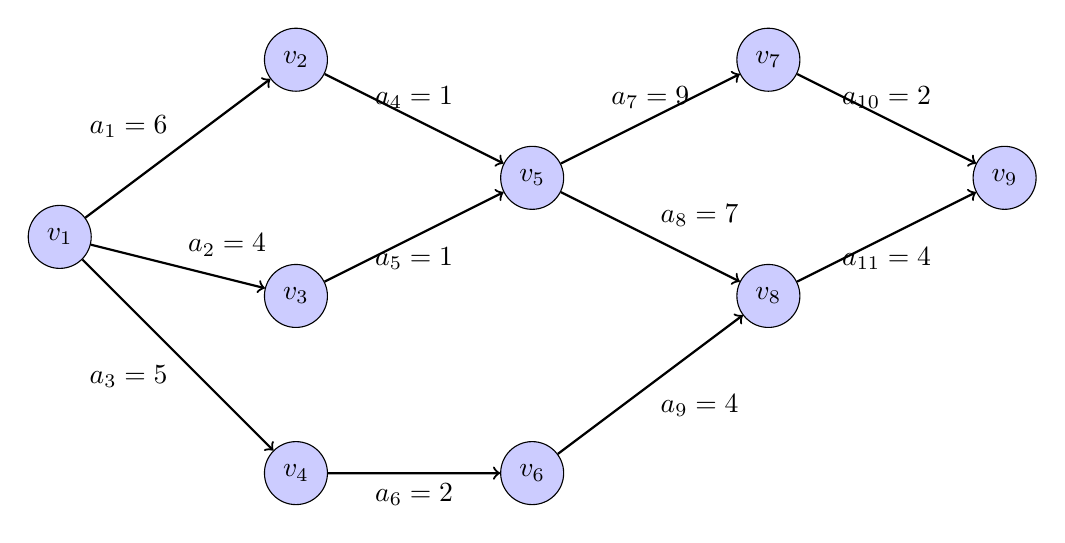
\begin{tikzpicture}[scale=1.5]
    % 定义节点样式
    \tikzstyle{vertex}=[circle,draw,minimum size=0.8cm,fill=blue!20]
    \tikzstyle{edge}=[thick,->]
    
    % 绘制顶点 - 按照用户图片的布局
    \node[vertex] (v1) at (0,0) {$v_1$};
    \node[vertex] (v2) at (2,1.5) {$v_2$};
    \node[vertex] (v3) at (2,-0.5) {$v_3$};
    \node[vertex] (v4) at (2,-2) {$v_4$};
    \node[vertex] (v5) at (4,0.5) {$v_5$};
    \node[vertex] (v6) at (4,-2) {$v_6$};
    \node[vertex] (v7) at (6,1.5) {$v_7$};
    \node[vertex] (v8) at (6,-0.5) {$v_8$};
    \node[vertex] (v9) at (8,0.5) {$v_9$};
    
    % 绘制边(活动)- 按照用户图片的连接方式
    \draw[edge] (v1) -- (v2) node[midway,above left] {$a_1=6$};
    \draw[edge] (v1) -- (v3) node[midway,above right] {$a_2=4$};
    \draw[edge] (v1) -- (v4) node[midway,below left] {$a_3=5$};
    \draw[edge] (v2) -- (v5) node[midway,above] {$a_4=1$};
    \draw[edge] (v3) -- (v5) node[midway,below] {$a_5=1$};
    \draw[edge] (v4) -- (v6) node[midway,below] {$a_6=2$};
    \draw[edge] (v5) -- (v7) node[midway,above] {$a_7=9$};
    \draw[edge] (v5) -- (v8) node[midway,above right] {$a_8=7$};
    \draw[edge] (v6) -- (v8) node[midway,below right] {$a_9=4$};
    \draw[edge] (v7) -- (v9) node[midway,above] {$a_{10}=2$};
    \draw[edge] (v8) -- (v9) node[midway,below] {$a_{11}=4$};
\end{tikzpicture}
\end{center}    

\textbf{关键路径算法步骤}:

\textbf{第一步:计算事件的最早发生时间$ve(i)$}

$ve(i)$表示事件$v_i$的最早发生时间,按拓扑序列从前向后计算:
\begin{align}
ve(1) &= 0 \quad \text{(源点)}\\
ve(2) &= ve(1) + 6 = 0 + 6 = 6\\
ve(3) &= ve(1) + 4 = 0 + 4 = 4\\
ve(4) &= ve(1) + 5 = 0 + 5 = 5\\
ve(5) &= \max\{ve(2) + 1, ve(3) + 1\} = \max\{6+1, 4+1\} = 7\\
ve(6) &= ve(4) + 2 = 5 + 2 = 7\\
ve(7) &= ve(5) + 9 = 7 + 9 = 16\\
ve(8) &= \max\{ve(5) + 7, ve(6) + 4\} = \max\{7+7, 7+4\} = 14\\
ve(9) &= \max\{ve(7) + 2, ve(8) + 4\} = \max\{16+2, 14+4\} = 18
\end{align}

\textbf{第二步:计算事件的最迟发生时间$vl(i)$}

$vl(i)$表示事件$v_i$的最迟发生时间,从汇点开始向前计算:
\begin{align}
vl(9) &= ve(9) = 18 \quad \text{(汇点)}\\
vl(8) &= vl(9) - 4 = 18 - 4 = 14\\
vl(7) &= vl(9) - 2 = 18 - 2 = 16\\
vl(6) &= vl(8) - 4 = 14 - 4 = 10\\
vl(5) &= \min\{vl(7) - 9, vl(8) - 7\} = \min\{16-9, 14-7\} = 7\\
vl(4) &= vl(6) - 2 = 10 - 2 = 8\\
vl(3) &= vl(5) - 1 = 7 - 1 = 6\\
vl(2) &= vl(5) - 1 = 7 - 1 = 6\\
vl(1) &= \min\{vl(2) - 6, vl(3) - 4, vl(4) - 5\} = \min\{6-6, 6-4, 8-5\} = 0
\end{align}

\textbf{第三步:计算活动的最早开始时间$ee(i)$和最迟开始时间$el(i)$}

对于活动$a_k: v_i \rightarrow v_j$,有:
\begin{itemize}
    \item $ee(k) = ve(i)$ (活动的最早开始时间等于起点事件的最早发生时间)
    \item $el(k) = vl(j) - dur(k)$ (活动的最迟开始时间等于终点事件的最迟发生时间减去活动持续时间)
\end{itemize}

\begin{center}
\begin{tabular}{|c|c|c|c|c|c|c|}
\hline
活动 & 起点 & 终点 & 持续时间 & $ee(k)$ & $el(k)$ & $el(k)-ee(k)$ \\
\hline
$a_1$ & $v_1$ & $v_2$ & 6 & $ve(1)=0$ & $vl(2)-6=6-6=0$ & 0 \\
\hline
$a_2$ & $v_1$ & $v_3$ & 4 & $ve(1)=0$ & $vl(3)-4=6-4=2$ & 2 \\
\hline
$a_3$ & $v_1$ & $v_4$ & 5 & $ve(1)=0$ & $vl(4)-5=8-5=3$ & 3 \\
\hline
$a_4$ & $v_2$ & $v_5$ & 1 & $ve(2)=6$ & $vl(5)-1=7-1=6$ & 0 \\
\hline
$a_5$ & $v_3$ & $v_5$ & 1 & $ve(3)=4$ & $vl(5)-1=7-1=6$ & 2 \\
\hline
$a_6$ & $v_4$ & $v_6$ & 2 & $ve(4)=5$ & $vl(6)-2=10-2=8$ & 3 \\
\hline
$a_7$ & $v_5$ & $v_7$ & 9 & $ve(5)=7$ & $vl(7)-9=16-9=7$ & 0 \\
\hline
$a_8$ & $v_5$ & $v_8$ & 7 & $ve(5)=7$ & $vl(8)-7=14-7=7$ & 0 \\
\hline
$a_9$ & $v_6$ & $v_8$ & 4 & $ve(6)=7$ & $vl(8)-4=14-4=10$ & 3 \\
\hline
$a_{10}$ & $v_7$ & $v_9$ & 2 & $ve(7)=16$ & $vl(9)-2=18-2=16$ & 0 \\
\hline
$a_{11}$ & $v_8$ & $v_9$ & 4 & $ve(8)=14$ & $vl(9)-4=18-4=14$ & 0 \\
\hline
\end{tabular}
\end{center}

\textbf{第四步:确定关键路径}

时间余量$d(k) = el(k) - ee(k) = 0$的活动为关键活动:$a_1, a_4, a_7, a_{10}$

\textbf{关键路径}:$v_1 \xrightarrow{a_1} v_2 \xrightarrow{a_4} v_5 \xrightarrow{a_7} v_7 \xrightarrow{a_{10}} v_9$

\textbf{另一条关键路径}:$v_1 \xrightarrow{a_1} v_2 \xrightarrow{a_4} v_5 \xrightarrow{a_8} v_8 \xrightarrow{a_{11}} v_9$

\textbf{工程最短完成时间}:18

\begin{center}
\begin{tikzpicture}[scale=1.5]
    % 定义节点样式
    \tikzstyle{vertex}=[circle,draw,minimum size=0.8cm,fill=blue!20]
    \tikzstyle{critical}=[circle,draw,minimum size=0.8cm,fill=green!30]
    \tikzstyle{critical1}=[circle,draw,minimum size=0.8cm,fill=red!30]
    \tikzstyle{critical2}=[circle,draw,minimum size=0.8cm,fill=blue!30]
    \tikzstyle{edge}=[thick,->]
    \tikzstyle{common_edge}=[very thick,->,green!70!black]
    \tikzstyle{critical_edge1}=[very thick,->,red]
    \tikzstyle{critical_edge2}=[very thick,->,blue]
    
    % 绘制顶点(用不同颜色标记不同关键路径)
    \node[critical] (v1) at (0,0) {$v_1$};        % 共同部分-绿色
    \node[critical] (v2) at (2,1.5) {$v_2$};      % 共同部分-绿色
    \node[vertex] (v3) at (2,-0.5) {$v_3$};       % 非关键顶点
    \node[vertex] (v4) at (2,-2) {$v_4$};         % 非关键顶点
    \node[critical] (v5) at (4,0.5) {$v_5$};      % 共同部分-绿色
    \node[vertex] (v6) at (4,-2) {$v_6$};         % 非关键顶点
    \node[critical1] (v7) at (6,1.5) {$v_7$};     % 关键路径1-红色
    \node[critical2] (v8) at (6,-0.5) {$v_8$};    % 关键路径2-蓝色
    \node[critical] (v9) at (8,0.5) {$v_9$};      % 汇聚点-绿色
    
    % 绘制边(用不同颜色标记不同关键路径)
    \draw[common_edge] (v1) -- (v2) node[midway,above left] {$a_1=6$};      % 共同部分-绿色
    \draw[edge] (v1) -- (v3) node[midway,above right] {$a_2=4$};             % 非关键边
    \draw[edge] (v1) -- (v4) node[midway,below left] {$a_3=5$};              % 非关键边
    \draw[common_edge] (v2) -- (v5) node[midway,above] {$a_4=1$};            % 共同部分-绿色
    \draw[edge] (v3) -- (v5) node[midway,below] {$a_5=1$};                   % 非关键边
    \draw[edge] (v4) -- (v6) node[midway,below] {$a_6=2$};                   % 非关键边
    \draw[critical_edge1] (v5) -- (v7) node[midway,above] {$a_7=9$};         % 关键路径1-红色
    \draw[critical_edge2] (v5) -- (v8) node[midway,above right] {$a_8=7$};   % 关键路径2-蓝色
    \draw[edge] (v6) -- (v8) node[midway,below right] {$a_9=4$};             % 非关键边
    \draw[critical_edge1] (v7) -- (v9) node[midway,above] {$a_{10}=2$};      % 关键路径1-红色
    \draw[critical_edge2] (v8) -- (v9) node[midway,below] {$a_{11}=4$};      % 关键路径2-蓝色
    
    \node at (4,-3) {\textbf{关键路径1:} $v_1 \rightarrow v_2 \rightarrow v_5 \rightarrow v_7 \rightarrow v_9$ \textcolor{red}{(红色)}};
    \node at (4,-3.5) {\textbf{关键路径2:} $v_1 \rightarrow v_2 \rightarrow v_5 \rightarrow v_8 \rightarrow v_9$ \textcolor{blue}{(蓝色)}};
    \node at (4,-4) {\textbf{共同部分:} $v_1 \rightarrow v_2 \rightarrow v_5$ \textcolor{green!70!black}{(绿色)}};
    \node at (4,-4.5) {\textbf{最短完成时间:18}};
\end{tikzpicture}
\end{center}

\textbf{关键路径算法公式总结}:

\begin{enumerate}
    \item \textbf{事件最早发生时间}:
    $$ve(j) = \max_{i \in P(j)} \{ve(i) + dur(i,j)\}$$
    其中$P(j)$表示事件$j$的所有前驱事件集合
    
    \item \textbf{事件最迟发生时间}:
    $$vl(i) = \min_{j \in S(i)} \{vl(j) - dur(i,j)\}$$
    其中$S(i)$表示事件$i$的所有后继事件集合
    
    \item \textbf{活动最早开始时间}:
    $$ee(k) = ve(i) \quad \text{活动}a_k: v_i \rightarrow v_j$$
    
    \item \textbf{活动最迟开始时间}:
    $$el(k) = vl(j) - dur(k) \quad \text{活动}a_k: v_i \rightarrow v_j$$
    
    \item \textbf{活动时间余量}:
    $$d(k) = el(k) - ee(k)$$
    
    \item \textbf{关键活动判定}:
    $$d(k) = 0 \Leftrightarrow \text{活动}a_k\text{是关键活动}$$
\end{enumerate}

\section{习题与解答}

\subsection{基础概念题}

\textbf{题目1}:已知无向图$G$有$n$个顶点$e$条边,求:
\begin{enumerate}
    \item 各顶点度数之和
    \item 若$G$是连通图,$e$的最小值和最大值
    \item 若$G$是完全图,求边数$e$
\end{enumerate}

\textbf{解答1}:
\begin{enumerate}
    \item 根据握手定理:$\sum_{i=0}^{n-1} TD(v_i) = 2e$
    \item 连通图:最小值$e_{min} = n-1$(树),最大值$e_{max} = \frac{n(n-1)}{2}$(完全图)
    \item 完全图:$e = \frac{n(n-1)}{2}$
\end{enumerate}

\textbf{题目2}:设有向图$G=(V,E)$,其中$V=\{v_1,v_2,v_3,v_4\}$,$E=\{\langle v_1,v_2\rangle, \langle v_1,v_3\rangle, \langle v_3,v_4\rangle, \langle v_4,v_1\rangle\}$,画出该图的邻接矩阵和邻接表。

\textbf{解答2}:

邻接矩阵:
$$
\begin{bmatrix}
0 & 1 & 1 & 0 \\
0 & 0 & 0 & 0 \\
0 & 0 & 0 & 1 \\
1 & 0 & 0 & 0
\end{bmatrix}
$$

邻接表:
\begin{align}
v_1 &: \rightarrow v_2 \rightarrow v_3 \rightarrow NULL \\
v_2 &: \rightarrow NULL \\
v_3 &: \rightarrow v_4 \rightarrow NULL \\
v_4 &: \rightarrow v_1 \rightarrow NULL
\end{align}

\subsection{算法应用题}

\textbf{题目3}:对下图从顶点$A$开始进行DFS和BFS遍历,写出遍历序列。

\begin{center}
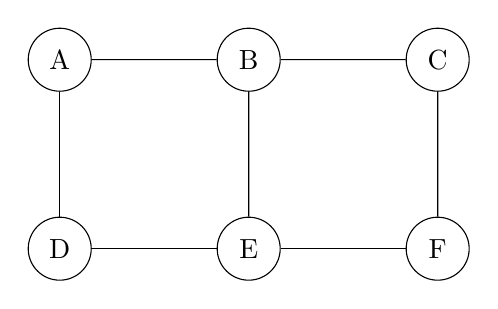
\begin{tikzpicture}[scale=1.2]
    \node[circle,draw,minimum size=0.8cm] (A) at (0,2) {A};
    \node[circle,draw,minimum size=0.8cm] (B) at (2,2) {B};
    \node[circle,draw,minimum size=0.8cm] (C) at (4,2) {C};
    \node[circle,draw,minimum size=0.8cm] (D) at (0,0) {D};
    \node[circle,draw,minimum size=0.8cm] (E) at (2,0) {E};
    \node[circle,draw,minimum size=0.8cm] (F) at (4,0) {F};
    
    \draw (A) -- (B);
    \draw (A) -- (D);
    \draw (B) -- (C);
    \draw (B) -- (E);
    \draw (C) -- (F);
    \draw (D) -- (E);
    \draw (E) -- (F);
\end{tikzpicture}
\end{center}

\textbf{解答3}:

DFS遍历序列(按字母顺序选择邻接点):$A \rightarrow B \rightarrow C \rightarrow F \rightarrow E \rightarrow D$

BFS遍历序列:$A \rightarrow B \rightarrow D \rightarrow C \rightarrow E \rightarrow F$

\textbf{题目4}:用Prim算法求下图的最小生成树,写出构造过程。

\begin{center}
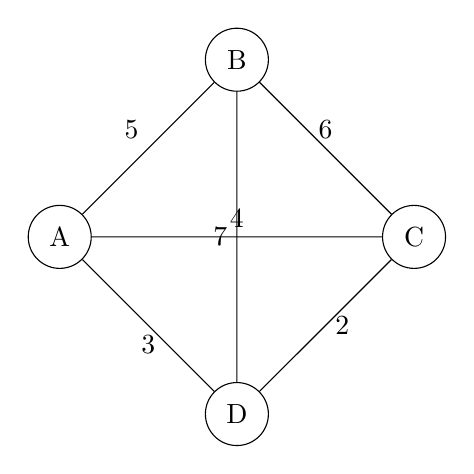
\begin{tikzpicture}[scale=1.5]
    \node[circle,draw,minimum size=0.8cm] (A) at (0,1.5) {A};
    \node[circle,draw,minimum size=0.8cm] (B) at (1.5,3) {B};
    \node[circle,draw,minimum size=0.8cm] (C) at (3,1.5) {C};
    \node[circle,draw,minimum size=0.8cm] (D) at (1.5,0) {D};
    
    \draw (A) -- node[above left] {5} (B);
    \draw (A) -- node[below] {3} (D);
    \draw (B) -- node[above] {6} (C);
    \draw (C) -- node[right] {2} (D);
    \draw (A) -- node[above] {4} (C);
    \draw (B) -- node[left] {7} (D);
\end{tikzpicture}
\end{center}

\textbf{解答4}:

从顶点$A$开始:

\begin{table}[h]
\centering
\begin{tabular}{|c|c|c|c|c|c|}
\hline
\textbf{步骤} & \textbf{U} & \textbf{选择的边} & \textbf{权值} & \textbf{lowcost更新} & \textbf{总权值} \\
\hline
初始 & $\{A\}$ & - & - & B:5, C:4, D:3 & 0 \\
\hline
1 & $\{A,D\}$ & $(A,D)$ & 3 & B:5, C:2 & 3 \\
\hline
2 & $\{A,D,C\}$ & $(D,C)$ & 2 & B:5 & 5 \\
\hline
3 & $\{A,D,C,B\}$ & $(A,B)$ & 5 & - & 10 \\
\hline
\end{tabular}
\end{table}

最小生成树包含边:$(A,D)$,$(D,C)$,$(A,B)$,总权值为10。

\textbf{题目5}:用Dijkstra算法求从顶点$S$到其他各顶点的最短路径。

\begin{center}
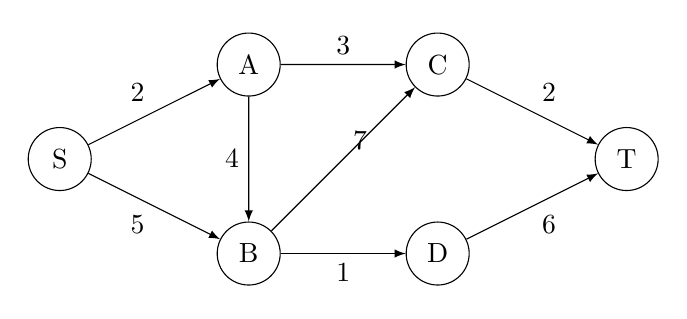
\begin{tikzpicture}[scale=1.2]
    \node[circle,draw,minimum size=0.8cm] (S) at (0,1) {S};
    \node[circle,draw,minimum size=0.8cm] (A) at (2,2) {A};
    \node[circle,draw,minimum size=0.8cm] (B) at (2,0) {B};
    \node[circle,draw,minimum size=0.8cm] (C) at (4,2) {C};
    \node[circle,draw,minimum size=0.8cm] (D) at (4,0) {D};
    \node[circle,draw,minimum size=0.8cm] (T) at (6,1) {T};
    
    \draw[-latex] (S) -- node[above left] {2} (A);
    \draw[-latex] (S) -- node[below left] {5} (B);
    \draw[-latex] (A) -- node[above] {3} (C);
    \draw[-latex] (A) -- node[left] {4} (B);
    \draw[-latex] (B) -- node[below] {1} (D);
    \draw[-latex] (C) -- node[above right] {2} (T);
    \draw[-latex] (D) -- node[below right] {6} (T);
    \draw[-latex] (B) -- node[above right] {7} (C);
\end{tikzpicture}
\end{center}

\textbf{解答5}:

Dijkstra算法执行过程:

\begin{table}[h]
\centering
\begin{tabular}{|c|c|c|c|c|c|c|c|}
\hline
\textbf{步骤} & \textbf{S集合} & \textbf{选择顶点} & \textbf{A} & \textbf{B} & \textbf{C} & \textbf{D} & \textbf{T} \\
\hline
初始 & $\{S\}$ & - & 2 & 5 & $\infty$ & $\infty$ & $\infty$ \\
\hline
1 & $\{S,A\}$ & A & - & 5 & 5 & $\infty$ & $\infty$ \\
\hline
2 & $\{S,A,B\}$ & B & - & - & 5 & 6 & $\infty$ \\
\hline
3 & $\{S,A,B,C\}$ & C & - & - & - & 6 & 7 \\
\hline
4 & $\{S,A,B,C,D\}$ & D & - & - & - & - & 7 \\
\hline
5 & $\{S,A,B,C,D,T\}$ & T & - & - & - & - & - \\
\hline
\end{tabular}
\end{table}

最短路径:
\begin{itemize}
    \item $S \rightarrow A$:距离2,路径:$S \rightarrow A$
    \item $S \rightarrow B$:距离5,路径:$S \rightarrow B$
    \item $S \rightarrow C$:距离5,路径:$S \rightarrow A \rightarrow C$
    \item $S \rightarrow D$:距离6,路径:$S \rightarrow B \rightarrow D$
    \item $S \rightarrow T$:距离7,路径:$S \rightarrow A \rightarrow C \rightarrow T$
\end{itemize}

\subsection{综合分析题}

\textbf{题目6}:某项目包含活动$A, B, C, D, E, F$,活动间的依赖关系如下:
\begin{itemize}
    \item 活动$A$:无前驱,持续时间3天
    \item 活动$B$:依赖$A$,持续时间4天
    \item 活动$C$:依赖$A$,持续时间2天
    \item 活动$D$:依赖$B, C$,持续时间5天
    \item 活动$E$:依赖$C$,持续时间3天
    \item 活动$F$:依赖$D, E$,持续时间2天
\end{itemize}

画出AOE网图,求关键路径和最短工期。

\textbf{解答6}:

AOE网图:

\begin{center}
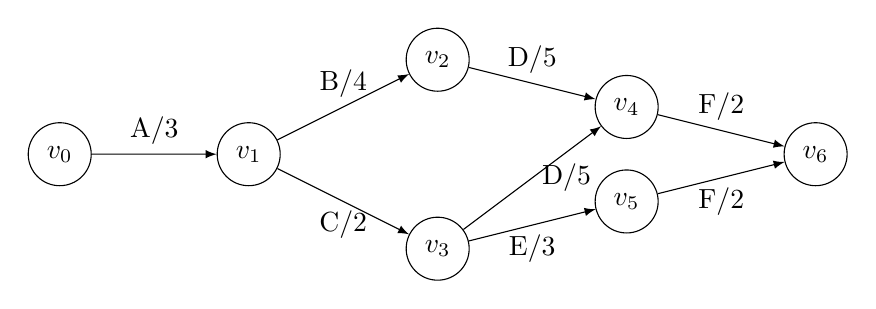
\begin{tikzpicture}[scale=1.2]
    \node[circle,draw,minimum size=0.8cm] (v0) at (0,1) {$v_0$};
    \node[circle,draw,minimum size=0.8cm] (v1) at (2,1) {$v_1$};
    \node[circle,draw,minimum size=0.8cm] (v2) at (4,2) {$v_2$};
    \node[circle,draw,minimum size=0.8cm] (v3) at (4,0) {$v_3$};
    \node[circle,draw,minimum size=0.8cm] (v4) at (6,1.5) {$v_4$};
    \node[circle,draw,minimum size=0.8cm] (v5) at (6,0.5) {$v_5$};
    \node[circle,draw,minimum size=0.8cm] (v6) at (8,1) {$v_6$};
    
    \draw[-latex] (v0) -- node[above] {A/3} (v1);
    \draw[-latex] (v1) -- node[above] {B/4} (v2);
    \draw[-latex] (v1) -- node[below] {C/2} (v3);
    \draw[-latex] (v2) -- node[above] {D/5} (v4);
    \draw[-latex] (v3) -- node[right] {D/5} (v4);
    \draw[-latex] (v3) -- node[below] {E/3} (v5);
    \draw[-latex] (v4) -- node[above] {F/2} (v6);
    \draw[-latex] (v5) -- node[below] {F/2} (v6);
\end{tikzpicture}
\end{center}

计算过程:

事件最早发生时间$ve$:
\begin{align}
ve[v_0] &= 0 \\
ve[v_1] &= 3 \\
ve[v_2] &= 7 \\
ve[v_3] &= 5 \\
ve[v_4] &= \max(12, 10) = 12 \\
ve[v_5] &= 8 \\
ve[v_6] &= \max(14, 10) = 14
\end{align}

事件最迟发生时间$vl$:
\begin{align}
vl[v_6] &= 14 \\
vl[v_5] &= 12 \\
vl[v_4] &= 12 \\
vl[v_3] &= \min(7, 9) = 7 \\
vl[v_2] &= 7 \\
vl[v_1] &= \min(3, 5) = 3 \\
vl[v_0] &= 0
\end{align}

关键活动判断($ee = el$):
\begin{itemize}
    \item 活动$A$:$ee = 0, el = 0$ ✓
    \item 活动$B$:$ee = 3, el = 3$ ✓
    \item 活动$C$:$ee = 3, el = 5$ ✗
    \item 活动$D$:$ee = 7, el = 7$ ✓
    \item 活动$E$:$ee = 5, el = 9$ ✗
    \item 活动$F$:$ee = 12, el = 12$ ✓
\end{itemize}

\textbf{结果}:
\begin{itemize}
    \item 关键路径:$v_0 \rightarrow v_1 \rightarrow v_2 \rightarrow v_4 \rightarrow v_6$
    \item 关键活动:$A \rightarrow B \rightarrow D \rightarrow F$
    \item 最短工期:14天
\end{itemize}

\subsection{计算题强化训练}

\textbf{题目7}:设无向图$G$有6个顶点,各顶点的度数分别为:2, 3, 3, 3, 4, 5。
\begin{enumerate}
    \item 验证是否满足握手定理
    \item 画出一个满足条件的图
    \item 该图最少有几个连通分量?
\end{enumerate}

\textbf{解答7}:
\begin{enumerate}
    \item 度数和:$2 + 3 + 3 + 3 + 4 + 5 = 20 = 2 \times 10$,满足握手定理,边数$e = 10$
    \item 可以构造满足条件的图(画图略)
    \item 最少1个连通分量(因为度数和为偶数且每个顶点度数都不为0)
\end{enumerate}

\textbf{题目8}:比较邻接矩阵和邻接表在以下操作的时间复杂度:
\begin{enumerate}
    \item 判断顶点$i$和$j$是否邻接
    \item 求顶点$i$的所有邻接点
    \item 在图中插入一个新顶点
    \item 删除顶点$i$
\end{enumerate}

\textbf{解答8}:

\begin{table}[h]
\centering
\begin{tabular}{|l|c|c|}
\hline
\textbf{操作} & \textbf{邻接矩阵} & \textbf{邻接表} \\
\hline
判断$(i,j)$是否邻接 & $O(1)$ & $O(度数)$ \\
\hline
求顶点$i$的所有邻接点 & $O(n)$ & $O(度数)$ \\
\hline
插入新顶点 & $O(n^2)$ & $O(1)$ \\
\hline
删除顶点$i$ & $O(n^2)$ & $O(n+e)$ \\
\hline
\end{tabular}
\end{table}

这些习题涵盖了图论的核心概念和算法,通过练习可以加深对知识点的理解和应用能力。建议结合教材和课堂讲解,多做手工模拟以掌握算法的执行过程。

\end{document} 